\documentclass{article}


% if you need to pass options to natbib, use, e.g.:
%     \PassOptionsToPackage{numbers, compress}{natbib}
% before loading neurips_2022


% ready for submission
% \usepackage{neurips_2022}


% to compile a preprint version, e.g., for submission to arXiv, add add the
% [preprint] option:
\usepackage[preprint]{neurips_2022}


% to compile a camera-ready version, add the [final] option, e.g.:
%     \usepackage[final]{neurips_2022}


% to avoid loading the natbib package, add option nonatbib:
%    \usepackage[nonatbib]{neurips_2022}


\usepackage[utf8]{inputenc} % allow utf-8 input
\usepackage[T1]{fontenc}    % use 8-bit T1 fonts
\usepackage{hyperref}       % hyperlinks
\usepackage{url}            % simple URL typesetting
\usepackage{booktabs}       % professional-quality tables
\usepackage{amsfonts}       % blackboard math symbols
\usepackage{amsmath, bm}
\usepackage{nicefrac}       % compact symbols for 1/2, etc.
\usepackage{microtype}      % microtypography
\usepackage{xcolor}         % colors
\usepackage{graphicx}

\title{
  Deep Bayesian Inference: \\ a natural coupling to deep neural networks
  % Deep Bayesian inference naturally couples to deep neural networks.
}


\author{%
  Wenfeng Feng\\
  % Department of Computer Science and Technology\\
  Henan Polytechnic University\\
  % Jiaozuo, Henan, China, 454003 \\
  \texttt{fengwf@hpu.edu.cn} \\
  \And
  Xin Zhang\\
  Henan Polytechnic University\\
  % Jiaozuo, Henan, China, 454003 \\
  \texttt{zhangxin@hpu.edu.cn} \\
}


\begin{document}


\maketitle


\begin{abstract}
  Deep
  where the observed evidence come from corresponding layer in deep neural network.
\end{abstract}


\section{Introduction}

Learning the conditional categorical distribution over a finite set of target labels or categories given the input observations plays an essential role in machine learning.
For example, in supervised learning, particular classification, we fit a conditional categorical distribution over a set of target classes given inputs. % $\bm{x}$ i.e. $p(y=c|\bm{x})$ % (P44 of \cite{murphy2022probabilistic}). ;\theta
In self-supervised learning, such as causal (or masked) language modeling, the joint probability distribution of the word sequence is factorized as the product of the conditional categorical distributions over the vocabulary of the next word (or the masked words) given the previous words (or the other unmasked words).
In reinforcement learning, a policy is represented as a conditional categorical distribution over a finite set of actions given input states or observations.
\textcolor{red}{add citations}

% A recently popular approach to unsupervised learning is known as self-supervised learning. In this approach, the task of unsupervised learning is transformed to supervised learning by creating a proxy supervised task. 
% For example, causal language modeling, predict the next word from a word sequence, masked language modeling, mask out words in a sentence and predict them given the surrounding context. 
% The resulting proxy task can also be viewed as a conditional model of the form $p(\bm{y}|\bm{x})$, where both outputs and inputs come from the unlabeled data.

The conditional categorical distribution over a finite set of possible target labels given the input observations is commonly represented as:
\begin{equation}
  p(\bm{y}|\bm{x}) = \bm{S}(\bm{f}(\bm{x})).
\end{equation}
In the above equation, $\bm{x}$ is the input observations, $y$ is a random variable that can take its values from a set of $n$ possible target labels, i.e. $\bm{y} \in \{y_1, \cdots, y_n\}$.
The function $\bm{f}$ embed and transform the input observations $\bm{x}$ to vectors in a $n$-dimensional real vector space $\mathbb{R}^n$.
These non-normalized vectors generated by function $\bm{f}$ are often called logits, which is then passed to Softmax function $\bm{S}$ that normalize the logits to a categorical probability distribution.

In modern machine learning, the function $\bm{f}$ is usually implemented by a deep neural network with multiple layers between inputs and outputs.
\textcolor{red}{Many deep neural network architectures evolved. CNN, Transformer, Mlp-mixer, etc.}

%The categorical distribution is a discrete probability distribution that describes the possible results of a random variable $y$ that can take on one of $C$ possible categories $\{1,\cdots,C\}$.
%The probability of each category is separately specified and works as parameters of the categorical distribution.
%In other words, $\theta_c = p(y=c), c \in \{1,\cdots,C\}$, where the parameters $\bm{\theta}=\{\theta_1, \cdots, \theta_c, \cdots, \theta_C\}$ are constrained so that $0 \le \theta_c \le 1$ and $\sum_{c=1}^C \theta_c = 1$.
% Note that there is no innate underlying ordering of the categories, but numerical labels are often attached for convenience in describing the distribution, (e.g. 1 to $C$).

A deep neural network architecture makes it easier to create deep representations, and learn multiple levels and aspects of input data features and concepts, layer by layer.
At every layer, the deep neural network learns a new, more abstract, higher-level, or different aspect representation of the input data features and concepts.
\url{https://www.researchgate.net/post/Why_Are_Deep_Networks_Better_Than_Shallow_Ones}

A deep neural network architecture can be formalized as a composition of functions $\bm{z} = f_{n} . f_{n-1} \ldots f_1(x_0) $.

既然f可以成为deep,softmax也可以成为deep

On the other hand, Bayesian inference is an iterative process utilizing Bayes' Theorem to deduce(infer) a probability distribution based on new observed data features coming in iteratively.

Since at each layer in a deep neural network, we get a new level or aspect representation of the input data,
they can serve as the new observed data in each Bayesian iteration.

In this sense, a Bayesian inference composed of multiple Bayesian iteration, where new observed data is provided by the corresponding layer in a deep neural network.
Thus, we call such architecture as Deep Bayesian Inference.

Rather than, all the different levels and aspects of input data feature can only be aggregated to the last layer of the neural network, and then are converted to categorical probabilities at the same time by the Softmax function,
they are converted to probability distribution layer by layer.

Therefore, we utilize Bayesian inference to convert the data features leaned by the neural network to likelihood, layer by layer.
Such a deep Bayesian inference architecture naturally coupled to the deep neural network, and stabilize,\textcolor{red}{Advantage of DBI}

We coupled DBI to three popular neural network architectures, Transformer, MlpMixer, ConvMixer, respectively.

The primary results of experiments show that:
1. Adding DBI to Transformer decreases the performance of classification. This may because Transformer capture global attention, and Softmax function in Transformer.
2. Adding DBI to MlpMixer could partially release overfitting problem.
3. Adding DBI to ConvMixer increase its performance obviously. This may be because convolution capture local attention layer by layer.

a layer learns something and then passes a representation to the next layer, which learns something else


The Bayesian inference provides a new approach to explanations of deep neural networks.

\section{Deep Bayesian Inference}



\begin{equation}
  p(y=c|\bm{x}) = \frac{p(\bm{x}|y=c)p(y=c)}{\sum_{c=1}^C p(\bm{x}|y=c)p(y=c)}
\end{equation}


When dealing with high-dimensional data, it is often useful to reduce the dimensionality by projecting it to a lower dimensional subspace which captures the "essence" of the data. (P46)

\subsection{Bayesian Inference}

Bayes theorem is a principle way to calculate a conditional probability.

The prior distribution is the available knowledge about the parameters in a statistical model, which is typically determined before any data are collected and observed. 

The observed evidence is expressed in terms of the likelihood function of the data given the parameters, is the conditional probability distribution $p(\bm{x}|\bm{\theta})$ of  the data $\bm{x}$ given parameters $\bm{\theta}$. 
In Bayesian inference, the likelihood $p(\bm{x}|\bm{\theta})$ comes into the posterior as a function of $\bm{\theta}$ for observed data $\bm{x}$. \citep{van2021bayesian}

At each Bayesian iteration, the likelihood function is provided by the output of the corresponding layer of the deep neural network.

Both prior distribution and likelihood function are combined via Bayes' Theorem in the form of the posterior distribution. The posterior distribution reflects the updated knowledge about the parameters, balancing the prior knowledge with the observed evidence.
The posterior distribution is a kind of weighted average (mean) of the prior distribution, where the likelihood function of the parameters are the weights. 

The obtained posterior results can then be used as the prior of the next iteration of Bayesian inference.

Bayesian inference is an iterative process utilizing Bayes' Theorem to deduce(infer) a probability distribution based on new observed data coming in iteratively \citep{harper2009replicator}.
Bayesian inference allows you to update your beliefs iteratively as new information(data) comes in. It works as follows: you have a prior belief about the distribution of your target, then, after you receive some new data, you can update your beliefs by calculating the posterior distribution by Bayes rule. Afterwards, we get even more data come in. So our posterior becomes the new prior. We can update the new prior with the likelihood derived from the new data and again we get a new posterior. This cycle can continue so long as new data comes in, so we can continuously updating our beliefs.

\url{https://towardsdatascience.com/probability-concepts-explained-bayesian-inference-for-parameter-estimation-90e8930e5348}


\subsection{Language Model}

A goal of language modeling is to learn the joint probability function of sequences of words in a language \citep{bengio2000neural}.


\url{https://www.inference.vc/implicit-bayesian-inference-in-sequence-models/}:
We can think of these one-step-ahead predictive distributions as implicitly performing Bayesian inference.

\begin{figure}
  \centering
  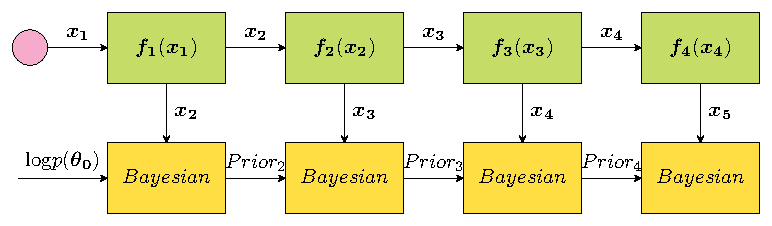
\includegraphics{dbi_diagram.pdf}
  % \fbox{\rule[-.5cm]{0cm}{4cm} \rule[-.5cm]{4cm}{0cm}}
  \caption{Sample figure caption.}
\end{figure}

\section{Deep Bayesian Inference Architecture}

DBI is a naturally extension of 

\paragraph{Advantage} 
Similar to auxiliary loss, DBI reduce the vanishing gradient problem for earlier layers, stabilize the training and is used as regularization.
\url{https://stats.stackexchange.com/questions/304699/what-is-auxiliary-loss-as-mentioned-in-pspnet-paper}

Deep generative models are used to estimate the likelihood of each observation and to create new samples from the underlying distribution.
Suppose the underlying distribution is a categorical distribution, whose parameters are $p_i, i \in [1, N]$.
Then the likelihood is defined as $P(p_i | c)$, where $c$ is the context observations.
The likelihood works as weights in a Bayesian iteration to update the prior belief.
(Ref: An introduction to deep generative modeling)



\subsection{Related Works}

\paragraph{Bayesian Neural Network}
A Bayesian neural network (BNN) is commonly defined as a stochastic artificial neural network trained using Bayesian inference \citep{jospin2022hands}.
While the prior distribution in BNN is taken over the possible model parameterization (is specified for each weight and bias),
the prior distribution of Deep Bayesian Inference is taken over the possible parameterization of data distribution.

\paragraph{Normalizing Flow}

\section{Experiments}
\paragraph{Experiment environment and setting}
We use Kaggle's free accessed GPUs to do our experiments. 
Kaggle provides a NVIDIA TESLA P100 GPU for each user which has 15.9GB memory, with a limit on each user's GPU use of 30 hours/week.
Due to the limitation of the hardware, we mainly do experiments on Tiny ImageNet, rather than ImageNet.

\subsection{Image Classification}

\paragraph{Vision Transformers and CNN}
\cite{dosovitskiy2020image}

\paragraph{Tiny ImageNet}
The Tiny ImageNet dataset is a modified subset of the original ImageNet dataset.
Here, there are 200 different classes instead of 1000 classes of ImageNet dataset,
with 100,000 training examples and 10,000 validation examples.
The resolution of the images is just 64x64 pixels.

\section{General formatting instructions}
\label{gen_inst}


The text must be confined within a rectangle 5.5~inches (33~picas) wide and
9~inches (54~picas) long. The left margin is 1.5~inch (9~picas).  Use 10~point
type with a vertical spacing (leading) of 11~points.  Times New Roman is the
preferred typeface throughout, and will be selected for you by default.
Paragraphs are separated by \nicefrac{1}{2}~line space (5.5 points), with no
indentation.


The paper title should be 17~point, initial caps/lower case, bold, centered
between two horizontal rules. The top rule should be 4~points thick and the
bottom rule should be 1~point thick. Allow \nicefrac{1}{4}~inch space above and
below the title to rules. All pages should start at 1~inch (6~picas) from the
top of the page.


For the final version, authors' names are set in boldface, and each name is
centered above the corresponding address. The lead author's name is to be listed
first (left-most), and the co-authors' names (if different address) are set to
follow. If there is only one co-author, list both author and co-author side by
side.


Please pay special attention to the instructions in Section \ref{others}
regarding figures, tables, acknowledgments, and references.


\section{Headings: first level}
\label{headings}


All headings should be lower case (except for first word and proper nouns),
flush left, and bold.


First-level headings should be in 12-point type.


\subsection{Headings: second level}


Second-level headings should be in 10-point type.


\subsubsection{Headings: third level}


Third-level headings should be in 10-point type.


\paragraph{Paragraphs}


There is also a \verb+\paragraph+ command available, which sets the heading in
bold, flush left, and inline with the text, with the heading followed by 1\,em
of space.


\section{Citations, figures, tables, references}
\label{others}


These instructions apply to everyone.


\subsection{Citations within the text}


The \verb+natbib+ package will be loaded for you by default.  Citations may be
author/year or numeric, as long as you maintain internal consistency.  As to the
format of the references themselves, any style is acceptable as long as it is
used consistently.


The documentation for \verb+natbib+ may be found at
\begin{center}
  \url{http://mirrors.ctan.org/macros/latex/contrib/natbib/natnotes.pdf}
\end{center}
Of note is the command \verb+\citet+, which produces citations appropriate for
use in inline text.  For example,
\begin{verbatim}
   \citet{hasselmo} investigated\dots
\end{verbatim}
produces
\begin{quote}
  Hasselmo, et al.\ (1995) investigated\dots
\end{quote}


If you wish to load the \verb+natbib+ package with options, you may add the
following before loading the \verb+neurips_2022+ package:
\begin{verbatim}
   \PassOptionsToPackage{options}{natbib}
\end{verbatim}


If \verb+natbib+ clashes with another package you load, you can add the optional
argument \verb+nonatbib+ when loading the style file:
\begin{verbatim}
   \usepackage[nonatbib]{neurips_2022}
\end{verbatim}


As submission is double blind, refer to your own published work in the third
person. That is, use ``In the previous work of Jones et al.\ [4],'' not ``In our
previous work [4].'' If you cite your other papers that are not widely available
(e.g., a journal paper under review), use anonymous author names in the
citation, e.g., an author of the form ``A.\ Anonymous.''


\subsection{Footnotes}


Footnotes should be used sparingly.  If you do require a footnote, indicate
footnotes with a number\footnote{Sample of the first footnote.} in the
text. Place the footnotes at the bottom of the page on which they appear.
Precede the footnote with a horizontal rule of 2~inches (12~picas).


Note that footnotes are properly typeset \emph{after} punctuation
marks.\footnote{As in this example.}


\subsection{Figures}


All artwork must be neat, clean, and legible. Lines should be dark enough for
purposes of reproduction. The figure number and caption always appear after the
figure. Place one line space before the figure caption and one line space after
the figure. The figure caption should be lower case (except for first word and
proper nouns); figures are numbered consecutively.


You may use color figures.  However, it is best for the figure captions and the
paper body to be legible if the paper is printed in either black/white or in
color.


\subsection{Tables}


All tables must be centered, neat, clean and legible.  The table number and
title always appear before the table.  See Table~\ref{sample-table}.


Place one line space before the table title, one line space after the
table title, and one line space after the table. The table title must
be lower case (except for first word and proper nouns); tables are
numbered consecutively.


Note that publication-quality tables \emph{do not contain vertical rules.} We
strongly suggest the use of the \verb+booktabs+ package, which allows for
typesetting high-quality, professional tables:
\begin{center}
  \url{https://www.ctan.org/pkg/booktabs}
\end{center}
This package was used to typeset Table~\ref{sample-table}.


\begin{table}
  \caption{Sample table title}
  \label{sample-table}
  \centering
  \begin{tabular}{lll}
    \toprule
    \multicolumn{2}{c}{Part}                   \\
    \cmidrule(r){1-2}
    Name     & Description     & Size ($\mu$m) \\
    \midrule
    Dendrite & Input terminal  & $\sim$100     \\
    Axon     & Output terminal & $\sim$10      \\
    Soma     & Cell body       & up to $10^6$  \\
    \bottomrule
  \end{tabular}
\end{table}


\section{Final instructions}


Do not change any aspects of the formatting parameters in the style files.  In
particular, do not modify the width or length of the rectangle the text should
fit into, and do not change font sizes (except perhaps in the
\textbf{References} section; see below). Please note that pages should be
numbered.


\section{Preparing PDF files}


Please prepare submission files with paper size ``US Letter,'' and not, for
example, ``A4.''


Fonts were the main cause of problems in the past years. Your PDF file must only
contain Type 1 or Embedded TrueType fonts. Here are a few instructions to
achieve this.


\begin{itemize}


\item You should directly generate PDF files using \verb+pdflatex+.


\item You can check which fonts a PDF files uses.  In Acrobat Reader, select the
  menu Files$>$Document Properties$>$Fonts and select Show All Fonts. You can
  also use the program \verb+pdffonts+ which comes with \verb+xpdf+ and is
  available out-of-the-box on most Linux machines.


\item The IEEE has recommendations for generating PDF files whose fonts are also
  acceptable for NeurIPS. Please see
  \url{http://www.emfield.org/icuwb2010/downloads/IEEE-PDF-SpecV32.pdf}


\item \verb+xfig+ "patterned" shapes are implemented with bitmap fonts.  Use
  "solid" shapes instead.


\item The \verb+\bbold+ package almost always uses bitmap fonts.  You should use
  the equivalent AMS Fonts:
\begin{verbatim}
   \usepackage{amsfonts}
\end{verbatim}
followed by, e.g., \verb+\mathbb{R}+, \verb+\mathbb{N}+, or \verb+\mathbb{C}+
for $\mathbb{R}$, $\mathbb{N}$ or $\mathbb{C}$.  You can also use the following
workaround for reals, natural and complex:
\begin{verbatim}
   \newcommand{\RR}{I\!\!R} %real numbers
   \newcommand{\Nat}{I\!\!N} %natural numbers
   \newcommand{\CC}{I\!\!\!\!C} %complex numbers
\end{verbatim}
Note that \verb+amsfonts+ is automatically loaded by the \verb+amssymb+ package.


\end{itemize}


If your file contains type 3 fonts or non embedded TrueType fonts, we will ask
you to fix it.


\subsection{Margins in \LaTeX{}}


Most of the margin problems come from figures positioned by hand using
\verb+\special+ or other commands. We suggest using the command
\verb+\includegraphics+ from the \verb+graphicx+ package. Always specify the
figure width as a multiple of the line width as in the example below:
\begin{verbatim}
   \usepackage[pdftex]{graphicx} ...
   \includegraphics[width=0.8\linewidth]{myfile.pdf}
\end{verbatim}
See Section 4.4 in the graphics bundle documentation
(\url{http://mirrors.ctan.org/macros/latex/required/graphics/grfguide.pdf})


A number of width problems arise when \LaTeX{} cannot properly hyphenate a
line. Please give LaTeX hyphenation hints using the \verb+\-+ command when
necessary.

\begin{ack}
Thanks Kaggle for providing free GPUs.
Do {\bf not} include this section in the anonymized submission, only in the final paper. You can use the \texttt{ack} environment provided in the style file to autmoatically hide this section in the anonymized submission.
\end{ack}


% \section*{References}

\bibliography{custom}
\bibliographystyle{acl_natbib}


%%%%%%%%%%%%%%%%%%%%%%%%%%%%%%%%%%%%%%%%%%%%%%%%%%%%%%%%%%%%
\section*{Checklist}


%%% BEGIN INSTRUCTIONS %%%
The checklist follows the references.  Please
read the checklist guidelines carefully for information on how to answer these
questions.  For each question, change the default \answerTODO{} to \answerYes{},
\answerNo{}, or \answerNA{}.  You are strongly encouraged to include a {\bf
justification to your answer}, either by referencing the appropriate section of
your paper or providing a brief inline description.  For example:
\begin{itemize}
  \item Did you include the license to the code and datasets? \answerYes{See Section~\ref{gen_inst}.}
  \item Did you include the license to the code and datasets? \answerNo{The code and the data are proprietary.}
  \item Did you include the license to the code and datasets? \answerNA{}
\end{itemize}
Please do not modify the questions and only use the provided macros for your
answers.  Note that the Checklist section does not count towards the page
limit.  In your paper, please delete this instructions block and only keep the
Checklist section heading above along with the questions/answers below.
%%% END INSTRUCTIONS %%%


\begin{enumerate}


\item For all authors...
\begin{enumerate}
  \item Do the main claims made in the abstract and introduction accurately reflect the paper's contributions and scope?
    \answerTODO{}
  \item Did you describe the limitations of your work?
    \answerTODO{}
  \item Did you discuss any potential negative societal impacts of your work?
    \answerTODO{}
  \item Have you read the ethics review guidelines and ensured that your paper conforms to them?
    \answerTODO{}
\end{enumerate}


\item If you are including theoretical results...
\begin{enumerate}
  \item Did you state the full set of assumptions of all theoretical results?
    \answerTODO{}
        \item Did you include complete proofs of all theoretical results?
    \answerTODO{}
\end{enumerate}


\item If you ran experiments...
\begin{enumerate}
  \item Did you include the code, data, and instructions needed to reproduce the main experimental results (either in the supplemental material or as a URL)?
    \answerTODO{}
  \item Did you specify all the training details (e.g., data splits, hyperparameters, how they were chosen)?
    \answerTODO{}
        \item Did you report error bars (e.g., with respect to the random seed after running experiments multiple times)?
    \answerTODO{}
        \item Did you include the total amount of compute and the type of resources used (e.g., type of GPUs, internal cluster, or cloud provider)?
    \answerTODO{}
\end{enumerate}


\item If you are using existing assets (e.g., code, data, models) or curating/releasing new assets...
\begin{enumerate}
  \item If your work uses existing assets, did you cite the creators?
    \answerTODO{}
  \item Did you mention the license of the assets?
    \answerTODO{}
  \item Did you include any new assets either in the supplemental material or as a URL?
    \answerTODO{}
  \item Did you discuss whether and how consent was obtained from people whose data you're using/curating?
    \answerTODO{}
  \item Did you discuss whether the data you are using/curating contains personally identifiable information or offensive content?
    \answerTODO{}
\end{enumerate}


\item If you used crowdsourcing or conducted research with human subjects...
\begin{enumerate}
  \item Did you include the full text of instructions given to participants and screenshots, if applicable?
    \answerTODO{}
  \item Did you describe any potential participant risks, with links to Institutional Review Board (IRB) approvals, if applicable?
    \answerTODO{}
  \item Did you include the estimated hourly wage paid to participants and the total amount spent on participant compensation?
    \answerTODO{}
\end{enumerate}


\end{enumerate}


%%%%%%%%%%%%%%%%%%%%%%%%%%%%%%%%%%%%%%%%%%%%%%%%%%%%%%%%%%%%


\end{document}